% Build in a temporary directory:
%   pdflatex -halt-on-error -output-directory=<temporary-directory> separated-product-junctions.tex
% The SVG and PNG are direct page exports of the resulting PDF.
\documentclass[tikz,border=12pt]{standalone}
\usepackage[T1]{fontenc}
\usepackage{lmodern,amsmath}
\usetikzlibrary{arrows.meta}
\definecolor{ink}{HTML}{183444}
\definecolor{blue}{HTML}{1B6780}
\definecolor{amber}{HTML}{AD601A}
\begin{document}
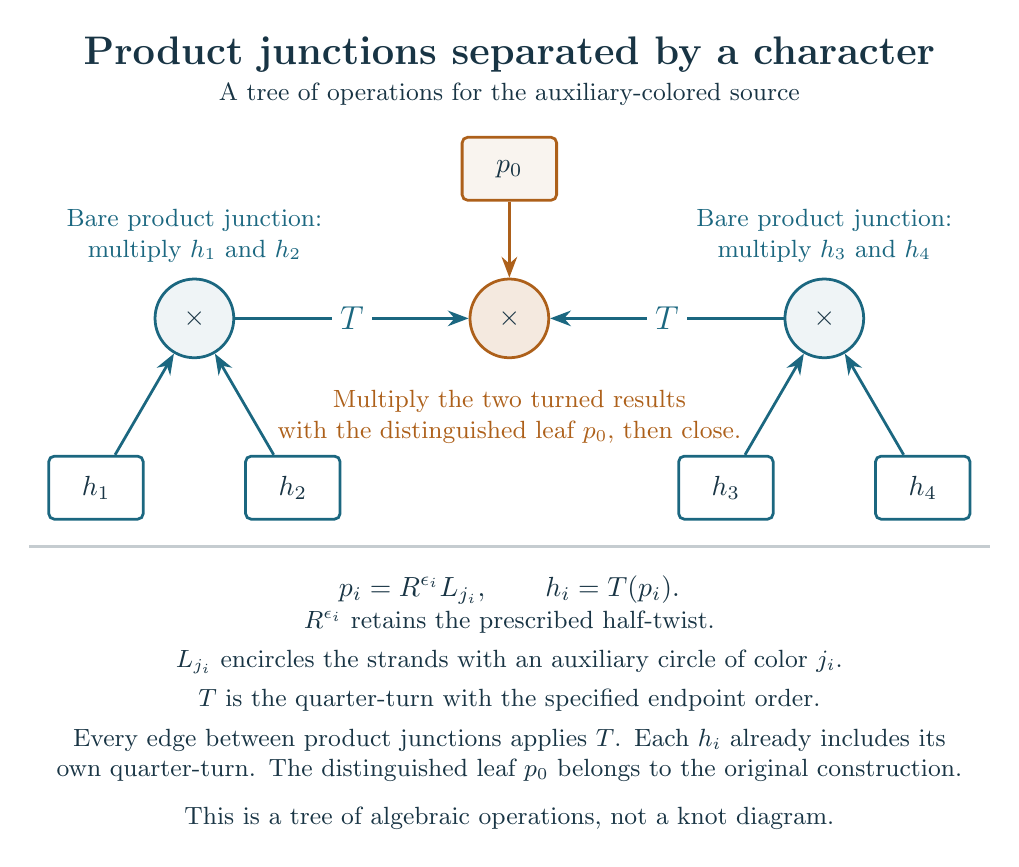
\begin{tikzpicture}[
  font=\sffamily,text=ink,line width=1pt,>=Stealth,
  junction/.style={circle,draw=blue,fill=blue!7,minimum size=10mm,inner sep=0pt},
  distinguished/.style={junction,draw=amber,fill=amber!14},
  leaf/.style={rounded corners=2pt,draw=blue,fill=white,
    minimum width=12mm,minimum height=8mm},
  turn/.style={fill=white,inner sep=3pt,font=\large,text=blue}
]
  \node[font=\Large\bfseries,align=center] at (0,4.45)
    {Product junctions separated by a character};
  \node[font=\small,align=center] at (0,3.95)
    {A tree of operations for the auxiliary-colored source};

  \node[junction] (left) at (-4,1.1) {$\times$};
  \node[distinguished] (center) at (0,1.1) {$\times$};
  \node[junction] (right) at (4,1.1) {$\times$};
  \node[leaf,draw=amber,fill=amber!7] (p0) at (0,3) {$p_0$};
  \node[leaf] (h1) at (-5.25,-1.05) {$h_1$};
  \node[leaf] (h2) at (-2.75,-1.05) {$h_2$};
  \node[leaf] (h3) at (2.75,-1.05) {$h_3$};
  \node[leaf] (h4) at (5.25,-1.05) {$h_4$};

  \draw[blue,->] (h1)--(left);
  \draw[blue,->] (h2)--(left);
  \draw[blue,->] (h3)--(right);
  \draw[blue,->] (h4)--(right);
  \draw[blue,->] (left)--node[turn]{$T$}(center);
  \draw[blue,->] (right)--node[turn]{$T$}(center);
  \draw[amber,->] (p0)--(center);

  \node[font=\small,align=center,text=blue] at (-4,2.15)
    {Bare product junction:\\multiply $h_1$ and $h_2$};
  \node[font=\small,align=center,text=blue] at (4,2.15)
    {Bare product junction:\\multiply $h_3$ and $h_4$};
  \node[font=\small,align=center,text=amber] at (0,-.15)
    {Multiply the two turned results\\with the distinguished leaf $p_0$, then close.};

  \draw[ink!25] (-6.1,-1.8)--(6.1,-1.8);
  \node[font=\normalsize,align=center] at (0,-2.35)
    {$\displaystyle p_i=R^{\epsilon_i}L_{j_i},\qquad h_i=T(p_i).$};
  \node[font=\small,align=center,text width=12cm] at (0,-3.25)
    {$R^{\epsilon_i}$ retains the prescribed half-twist.\\[3pt]
     $L_{j_i}$ encircles the strands with an auxiliary circle of color $j_i$.\\[3pt]
     $T$ is the quarter-turn with the specified endpoint order.};
  \node[font=\small,align=center,text width=12cm] at (0,-4.45)
    {Every edge between product junctions applies $T$.
     Each $h_i$ already includes its own quarter-turn.
     The distinguished leaf $p_0$ belongs to the original construction.};
  \node[font=\small,align=center] at (0,-5.25)
    {This is a tree of algebraic operations, not a knot diagram.};
\end{tikzpicture}
\end{document}
